\documentclass[10pt]{article}
\usepackage[utf8]{inputenc}

\title{Multi-scale analysis for depth estimation}
\author{Vasileios Gkolemis, Anastasios Delopoulos}
\date{January 2020}

% \usepackage{geometry}
%  \geometry{
%  left=20mm,
%  top=20mm,
%  }

\usepackage{mathtools}
\usepackage{amsmath}
\usepackage{amsfonts}
\usepackage{xfrac}

\usepackage{svg}
\usepackage{csvsimple}

\usepackage{algorithm}
\usepackage{algpseudocode}

\usepackage{graphicx}
\usepackage{caption}
\usepackage{subcaption}
\graphicspath{ {./figures/} }

\begin{document}

\maketitle

\section{Introduction}

Stereo vision forms a particular case of the general 3D reconstruction problem. Stereo cameras share the same orientation while their centre is displaced horizontally by a distance $B$. The following relation expresses stereo vision's 3D geometry:

\begin{equation} \label{eq:stereo_geometry}
z = f\frac{B}{d}
\end{equation}

where $z$ is the distance from the camera level (depth), $f$ is the focal length of the camera and $d$ is the disparity; the horizontal difference between the object's projection in each of the stereo cameras. Let's define the stereo pair as $X = (X^L, X^R)$. Finding all correspondences $X^L(x,y) \leftrightarrow X^R(x-d, y), \forall (x,y)$ reveals the disparity image $Y$, which is the target of the problem.

%%%%%%%%%%%%%%%%%%%%%%%%%%%%%%%%%%%%%%%%%%%%%%%%%%%%%%%%%%%%
\section{Related work}

Reconstructing the three dimensional geometry from a set of $2D$ images is a core problem of computer vision. Stereo reconstruction is a predominant technique of the aforementioned domain and has been heavily studied over years \cite{Barnard1982ComputationalStereo, Brown2003}. Scharstein and Szeliski \cite{Scharstein2001AAlgorithms} propose a general taxonomy framework for describing and analysing any stereo vision algorithm in four steps: matching cost computation, cost aggregation, disparity computation/optimisation and disparity refinement.

The matching cost computation realises a dissimilarity measurement between each pixel on reference image and all possible corresponding locations. Quite a lot of metrics of dissimilarity have been proposed, including  absolute difference, squared difference, cross correlation and hamming distance. Dissimilarity metrics can be applied on many different local descriptors, such as LoG, CENSUS \cite{Zabih1996ACorrespondence} and BRIEF \cite{Calonder2010}. Mutual Information \cite{Viola1997} proposes a rather different metric based on the entropy of histograms of correnspondent locations. An extensive evaluation of different matching cost computation strategies has been proposed by \cite{Hirschmuller2007}. Initial matching costs are error prone due to the intense locality of information. Initial estimates need to get optimized by methods taking into account global image information. This can be accomplished through graph cuts \cite{Kolmogorov, Boykov2001} and belief propagation \cite{Klaus2006}. Semi-Global-Matching (SGM) \cite{Hirschmuller2008StereoInformation} attempts to minimize a global energy function.

Stereo vision methods are evaluated on datasets containing ground truth depth or disparity for stereo pairs. Middlebury \cite{Scharstein2014} contains indoor scenes. KITTI \cite{Menze2015ISA, Menze2018JPRS} is a larger dataset with outdoor scenes and ground truth labels collected from LIDAR on a moving vehicle. Mayer et. al \cite{Mayer2016ALD} created a big synthetic dataset for training big machine learning models.

Deep convolutional networks show great success on stereo vision problems. Intial deep learning proposals focused on matching cost compuation. Zagoruyko et. al \cite{Zagoruyko2015LearningNetworks} proposed a deep convolutional neural network for comparing image patches. \v{Z}bontar and LeCun \cite{Zbontar_2015_CVPR} trained a deep network for predicting the initial matching scores on $9x9$ image patches, followed by traditional aggregation and refinement methods. Luo et. al \cite{Luo2016EfficientMatching} treated matching scores estimation as a multi-label classification problem.

Shaked and Wolf [12] introduce an initial disparity prediction network pooling global information from cost volume

%%%%%%%%%%%%%%%%%%%%%%%%%%%%%%%%%%%%%%%%%%%%%%%%%%%%%%%%%%%%%%%%
\section{Multiscale analysis}

Disparity estimation is based on the hypothesis that the local context of correspondent points is similar. If we define as $P_{n \times n}[x,y]$ the  $n \times n$ square patch centered at $X[x,y]$ and $g(\cdot)$ a metric of patch similarity, then we assume that:

\begin{equation}
\begin{gathered} \label{eq:similarity_hypothesis}
    g(P^L_{n \times n}[x,y], P^R_{n \times n}[x-d^*,y]) > g(P^L_{n \times n}[x,y], P^R_{n \times n}[x-d,y]) \\
    \forall d \in [0,D] : d \neq d^*, \text{where $d* = Y[x,y]$}
\end{gathered}
\end{equation}

For hypothesis \ref{eq:similarity_hypothesis} to hold, we must choose carefully two critical factors that depend on the specific properties of the points under comparison. Firstly, we must select the patch size correctly (i.e. a textureless region requires a large patch size, whereas a region with many features and multiple-depth objects in the background requires a small patch). Secondly, we must select the scale of the image correctly, so that the similarity measure $g$ be able to detect and match the unique features inside the patch. Since it is impossible to know a priori the correct patch size and the correct processing scale for each image point, we choose to design a deep learning architecture that incorporates the machinery of multiscale analysis. In figure \ref{fig:multiscale_importance_2D}, we design a simple artificial example to show the importance of multiscale processing, by attempting to match patches with different properties (i.e. one scenario requires coarse-scale processing, whereas the other fine-scale). Finally, apart from tackling the aforementioned crucial questions successfully, the multiscale approach offers another attractive advantage; it leads to an agile CNN architecture that can be readjusted between efficiency and accuracy, at the inference phase. If we seek for efficiency, we can tune the network to operate at fewer scales and vice-versa if accuracy is the priority. This tuning can be done through hyperparameters, without the need to retrain the initial CNN.

After, obtaining such multiscale similarity estimations, we implement a recursive $3D$ module for merging the different disparity estimations into a final prediction. In general, our cnn architecture follows the next to designing principles:

\begin{itemize}
    \item Implements comparisons at a range of different scales
    \item Merges different comparison scales, adopting the one with the most accurate info
\end{itemize}

%%%%%%%%%%%%%%%%%%%%%%%%%%%%%%%%%%%%%%%%%%%%%%%%%%%%%%%%%%%%%%%%%
%%%%%%%%%%%%%%% Multiscale 2d importance %%%%%%%%%%%%%%%%%%%%%%%%
\begin{figure*}[t]
\makebox[\textwidth][c]{
\begin{subfigure}[t]{0.53\textwidth}
    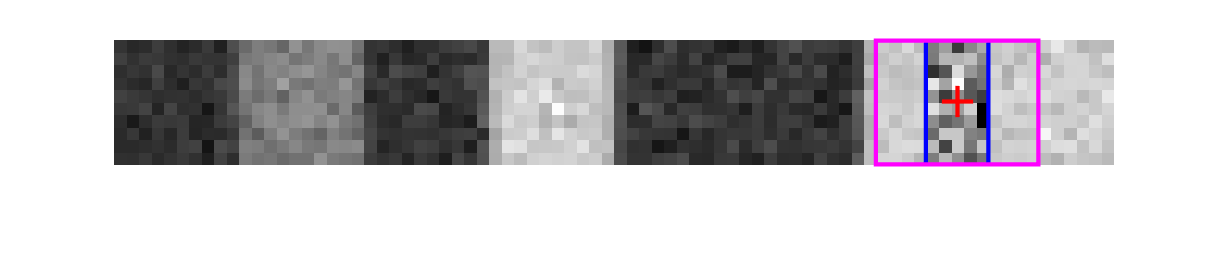
\includegraphics[width=\textwidth]{paper/latex/figures/high_resolution_success_imL_fine.png}
    \vspace{-15pt}
\end{subfigure}
\begin{subfigure}[t]{0.53\textwidth}
    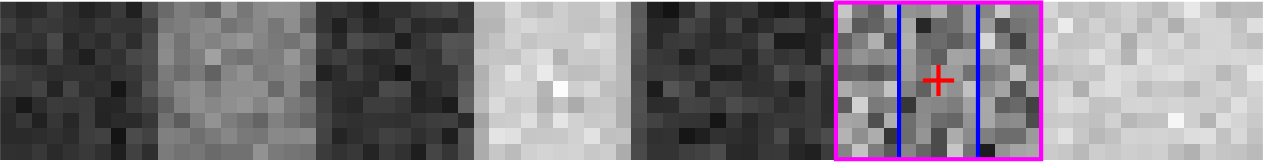
\includegraphics[width=\textwidth]{paper/latex/figures/low_resolution_success_imL_fine.png}\\
    \vspace{-15pt}
\end{subfigure}
}

\makebox[\textwidth][c]{
\begin{subfigure}[t]{0.53\textwidth}
    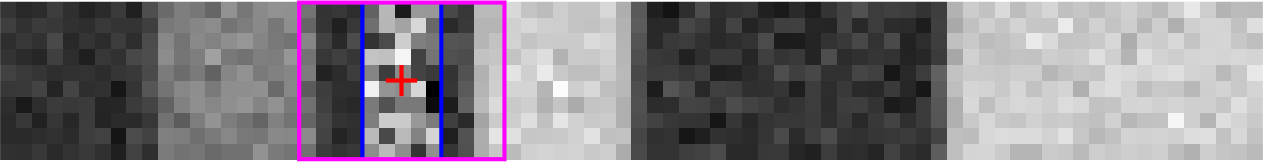
\includegraphics[width=\textwidth]{paper/latex/figures/high_resolution_success_imR_fine.png}
    \vspace{-15pt}
\end{subfigure}
\begin{subfigure}[t]{0.53\textwidth}
    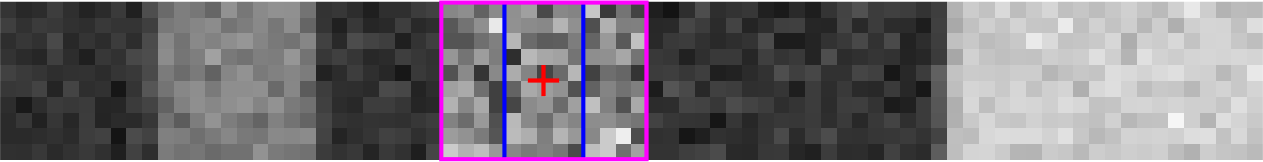
\includegraphics[width=\textwidth]{paper/latex/figures/low_resolution_success_imR_fine.png}\\
    \vspace{-15pt}
\end{subfigure}
}

\makebox[\textwidth][c]{
\begin{subfigure}[t]{0.53\textwidth}
    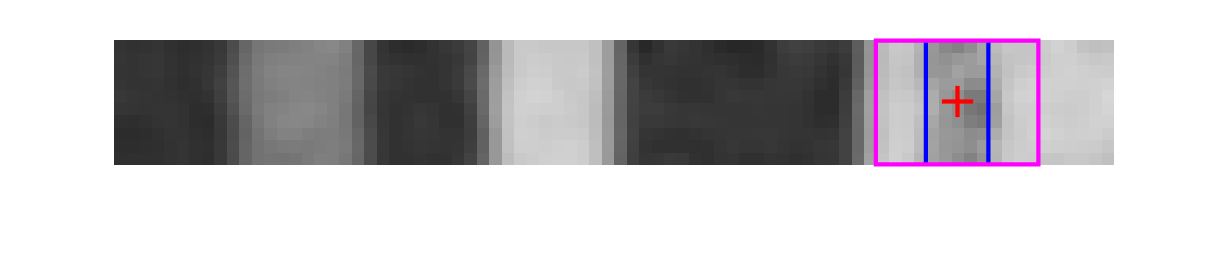
\includegraphics[width=\textwidth]{paper/latex/figures/high_resolution_success_imL_coarse.png}
    \vspace{-15pt}
\end{subfigure}
\begin{subfigure}[t]{0.53\textwidth}
    
\includegraphics[width=\textwidth]{paper/latex/figures/low_resolution_success_imL_coarse.png}\\
    \vspace{-15pt}
\end{subfigure}
}

\makebox[\textwidth][c]{
\begin{subfigure}[t]{0.53\textwidth}
    
\includegraphics[width=\textwidth]{paper/latex/figures/high_resolution_success_imR_coarse.png}
    \vspace{-5pt}
\end{subfigure}
\begin{subfigure}[t]{0.53\textwidth}
    
\includegraphics[width=\textwidth]{paper/latex/figures/low_resolution_success_imR_coarse.png}\\
    \vspace{-5pt}
\end{subfigure}
}

\makebox[\textwidth][c]{
\begin{subfigure}[t]{0.54\textwidth}
    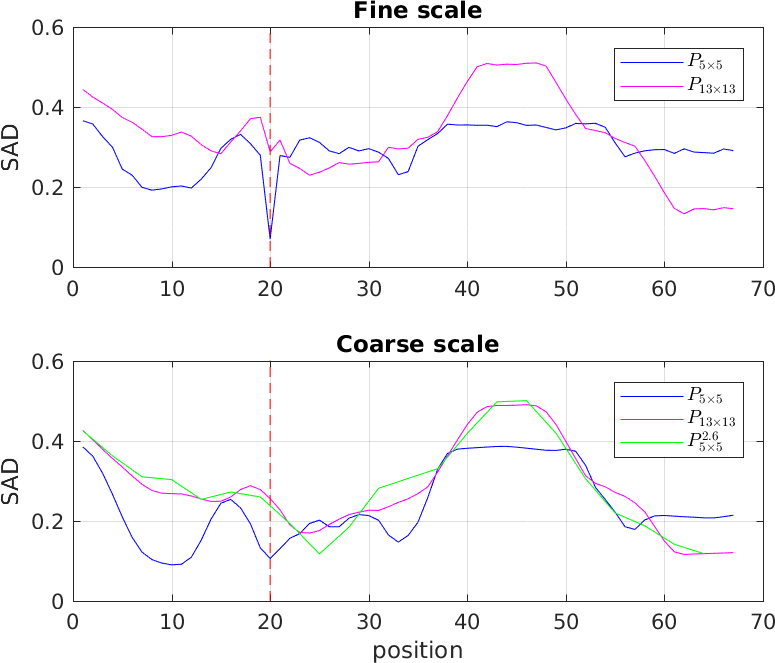
\includegraphics[width=\textwidth]{paper/latex/figures/high_resolution_success_graph.png}
    \vspace{-10pt}
\end{subfigure}
\begin{subfigure}[t]{0.54\textwidth}
    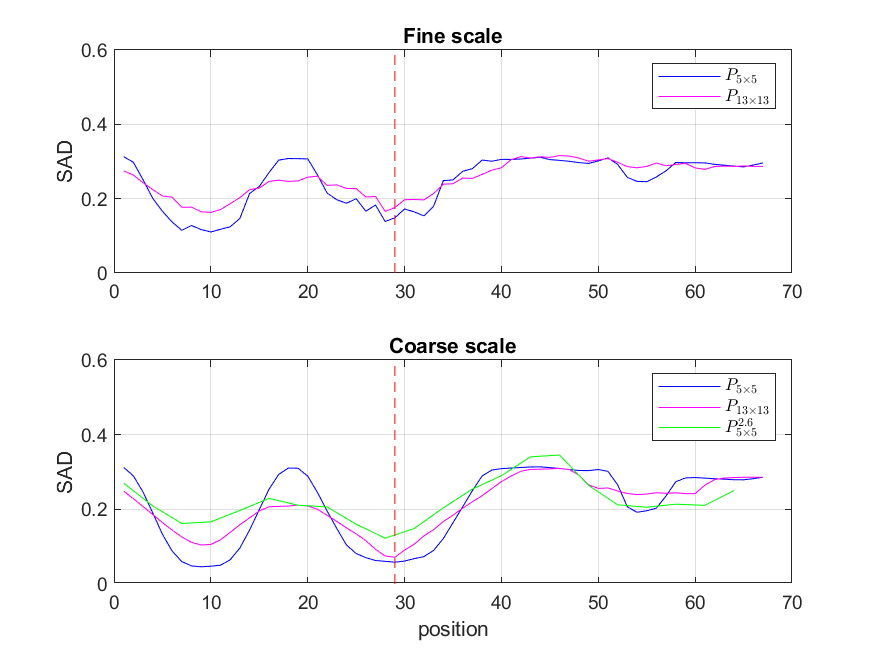
\includegraphics[width=\textwidth]{paper/latex/figures/low_resolution_success_graph.png}\\
    \vspace{-10pt}
\end{subfigure}
}
\vspace{-15pt}
\caption{In this figure, we draw a simple artificial example to demonstrate the importance of multiscale patch comparison. In the left column, the fine scale image combined with a small patch size $P_{5 \times 5}$ leads to an accurate disparity curve, whereas in the right example, this happens through the coarse scale and the bigger patch $P_{13 \times 13}$. In the right example, we can observe, that we can approach the same disparity curve by applying a small patch size ($5 \times 5$) after downsampling the coarse scale image at a rate $\sfrac{13}{5}$. This example verifies that instead of keep changing the patch size, we can keep it fixed and apply it to a scale-space pyramid of the stereo pair.}
\label{fig:multiscale_importance_2D}  
\vspace{-3pt}      
\end{figure*}
%%%%%%%%%%%%%%%%%%%%%%%%%%%%%%%%%%%%%%%%%%%%%%%%%%%%%%%%%%%%%%%%
%%%%%%%%%%%%%%%%%%%%%%%%%%%%%%%%%%%%%%%%%%%%%%%%%%%%%%%%%%%%%%%%

\subsection{MSNet architecture}

In this section, we describe the architecture of MSNet. MSNet comprises of specific subparts, each one with a specific role in the estimation of depth. We name as $f_*$ the parts that contain learnable parameters (i.e. CNN) and $g_*$ the parts without learned parts. For the best understanding of our description, it is crucial to pay attention to the table \ref{tab:entity_description} and to figure \ref{fig:cnn_architecture}.

\subsubsection{Downscaling stereo pair - $g_1$}

$g_1^t : \mathbb{R}^{H \times W} \rightarrow \mathbb{R}^{\sfrac{H}{t} \times \sfrac{W}{t}}$ creates a downscaled stereo pair, where $t$ is the downscaling factor. 

$$(X^{L,t}, X^{R,t}) = (g_1^t(X^L), g_1^t(X^R)) $$

Specifically, $g_1^t$ convolves the stereo image $X$ with a gaussian kernel 

$$k(x, y, \sigma) = \frac{1}{2\pi\sigma^2} \cdot e^{\sfrac{-(x^2 + y^2)}{2\sigma^2}}$$ of size $N = 2 * \lceil 4*\sigma + 0.5 \rceil - 1, \sigma = \sfrac{t}{3}$ and afterwards applies bilinear downsampling. In our work, the scales $t$ are set to be powers of 2 (i.e $ T = \{ 2^2, 2^3, 2^4, 2^5 \}$) but in general they can be defined to be any positive number. 


\subsubsection{Feature extraction - $f_1$}

The module $f_1: \mathbb{R}^{H \times W \times 3} \rightarrow \mathbb{R}^{H \times W \times K}$ is the CNN responsible for extracting local features for each point of the stereo images. This process is done separately for each stereo image and each scale.

$$ (X^{L,t}_{desc}, X^{R,t}_{desc}) = (f_1(X^{L,t}), f_1(X^{R, t})), \forall t$$

\subsubsection{Comparison volume - $g_2$}

The comparison volume $g_2: (\mathbb{R}^{H \times W \times K}, \mathbb{R}^{H \times W \times K}) \rightarrow \mathbb{R}^{D \times H \times W \times K'}$ is used as a helping step for zipping comparison information into a 3D tensor. Normally, the comparison volume is formed by simply concatenating the descriptors for each disparity position. This approach introduces significant redundancy; the comparison volume with dimensionality $D \times H \times W \times 2K$ is builded by repeting  $H \times W \times 2K$ unique values. For keeping the memory space and reduce redundancy, we design a new comparison metric between two scalar features:

$$ g_2: \mathbb{R}^2 \rightarrow \mathbb{R}: g_2(a_1, a_2) = \frac{|a_1| + |a_2|}{2} \cdot e^{-|a_1 - a_2|} $$

The second term $e^{-|a_1 - a_2|} \in (0,1]$ measures whether the specific feature is found in both image patches and the first term $\frac{|a_1| + |a_2|}{2}$ whether the feature is strong in each patch (i.e. $0$ is the weakest value for the feature). With this formulation, we avoid redundancy, since all values entering the comparison volume indicate whether a specific feature has been located in both patches under comparison.
Finally, we concatenate the raw left image $X^L$ along the axis $d$ of the comparison volume, so to save the local context information for the forthcoming layers.

\begin{equation}
\begin{gathered} \label{eq:comparison_volume}
    C^t[d, x, y, i] = g_2( X^{L, t}_{desc}[x,y,i], X^{R, t}_{desc}[x-d,y, i]) \\
    C^t \leftarrow X^{L, t} \oplus C^t
\end{gathered}
\end{equation}

\subsubsection{Comparison volume processing - $f_2$}


\subsubsection{Multiscale fusion - $f_3$}

This module is responsible for exploiting information from different scales and merge it in a single comparison volume. The procedure takes place recursively in pairs of two, from coarse to fine scales; a coarse (low resolution) scale is getting merged with a fine (higher resolution) until the highest resolution is reached. The goal of the learnable module $f_3$ is to understand which scale includes the most reliable information and carry it forward to the next level. After multiscale fusion has been completed, the output tensor $Q^{\{t_0, t_1, \cdot \cdot \cdot, t_n\}}$, which has the same dimensions as $Q^{t_0}$, contains accumulated information from all single-scale tensors. 

Apart from the learnable $f_3$ module, a trilinear upsampling layer 

$$g_3^t: \mathbb{R}^{D \times H \times W \times K} \rightarrow \mathbb{R}^{tD \times tH \times tW \times K}$$ where $t$ represents the upsampling factor, is being used. 

Equation \ref{eq:two_scale_fusion} explains how the scale $i$ is being adopted in the multiscale fusion procedure and the end-to-end explanation of the algorithm is given in \ref{alg:multi_scale_fusion}:

\begin{equation} \label{eq:two_scale_fusion}
Q^{ \{ t_i, \cdot \cdot \cdot, t_{n} \} } = f_3(Q^{t_i} \oplus g_3^{\sfrac{t_i}{t_{i-1}} }(Q^{ \{ t_{i-1}, \cdot \cdot \cdot, t_n \} }))
\end{equation}


\begin{algorithm}
\caption{Multi-scale fusion}\label{alg:multi_scale_fusion}
\begin{algorithmic}[1]
\Procedure{multi scale fusion}{$ Q^{t_0}, Q^{t_1}, \cdot \cdot \cdot, Q^{t_n} $} $\rightarrow Q^{\{t_0, t_1, \cdot \cdot \cdot, t_n\}}$ 
\State $Q \gets Q^{t_n}$ \Comment{Initialize}
\For { \texttt{i=n-1;-1;0} }
\State $Q \gets g_3^{\sfrac{ t_{i+1} }{ t_i } }(Q)$ \Comment{3D Upsampling}
\State $Q \gets Q^{t_i} \oplus Q$ \Comment{Concatenation}
\State $Q \gets f_3(Q)$ \Comment{Merge information}
\EndFor
\State \Return $Q^{\{t_0, t_1, \cdot \cdot \cdot, t_n\}} \gets Q$ \Comment{Result}
\EndProcedure
\end{algorithmic}
\end{algorithm}


\subsubsection{Final prediction - $f_4$ and softargmax}

The module $f_4: \mathbb{R}^{D \times H \times W \times K} \rightarrow \mathbb{R}^{D \times H \times W}$ is responsible for predicting a vector of probabilities for each possible disparity:

$$S^{\{ t_0, \cdot \cdot \cdot, t_n \}} = f_4(Q^{\{t_0, t_1, \cdot \cdot \cdot, t_n\}})$$

A softmax operator applied alond the disparity dimension produces the final prediction:

$$Y^{\{ t_0, \cdot \cdot \cdot, t_n \}} = softargmax_d(S^{\{ t_0, \cdot \cdot \cdot, t_n \}})$$

\subsubsection{Putting all pieces together}

MSNet comprises of 4 CNN modules - $f_1, f_2, f_3, f_4$, which are repeated for extracting information at multiple scales and then combine it for producing a single prediction image. At training time, we fix the list of scales to $T = \{ 2^0, 2^1, 2^2, 2^3 \}$. At test time, this list can be changed depending on the specific application needs. For example, if the application lacks computational resources and targets to a quick and rough depth estimation, the scale-list can be set to $T = \{ 16, 32, 64\}$. Vice-versa, if the application needs accuracy and high-resolution detail the list can be set to $T = \{1, 2, 4, 8 \}$.


\subsection{Cnn architectures}

In this section we present the specific cnn architectures used as the learnable parts of our model. 

\begin{figure}
    \centering
    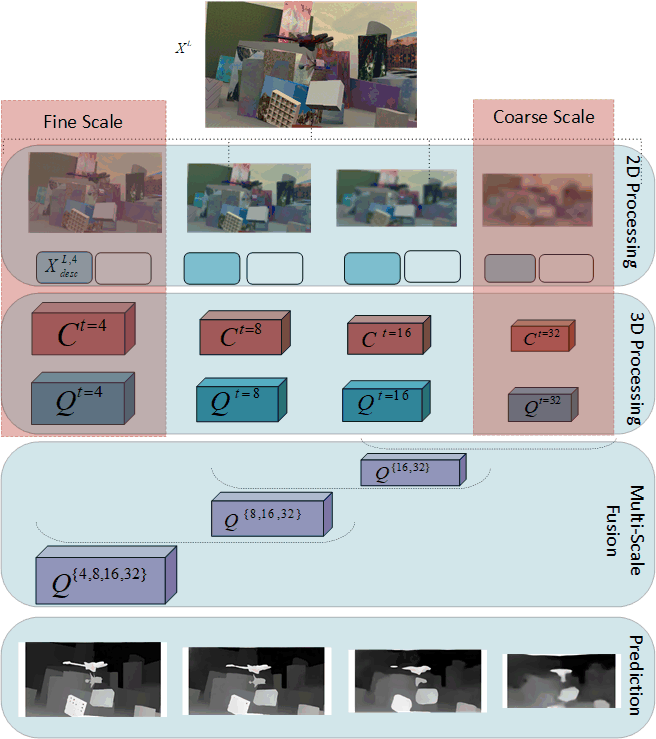
\includegraphics[width = \textwidth]{paper/latex/figures/stereo_architecture.png}
    \caption{Scale fusion network overview. Its main constructive blocks are the horizontal pipelines (green colour) representing end-to-end predictions at specific scale $\sigma$ and the vertical pipelines (grey colour) representing the pair-scales fusion at similarity matrix level. The red-coloured blocks are the learned parts of our architecture, while the yellow coloured ones are hand-crafted layers.}
    \label{fig:cnn_architecture}
\end{figure}

\begin{table}[]
    \centering
    \begin{tabular}{ l|c|c }
    Description & Symbol & Set \rule{0pt}{2ex}\\
    
    \hline
    \multicolumn{3}{c}{ \textbf{Definitions} } \rule{0pt}{2.4ex}\\
    \hline
    
    Raw image & $X^L, X^R$ & $\mathbb{R}^{H \times W \times 3}$ \rule{0pt}{2.5ex} \\
    
    Ground truth & $Y$ & $\mathbb{R}^{H \times W}$ \rule{0pt}{2.5ex} \\
    
    \hline
    \multicolumn{3}{c}{ \textbf{Single-Scale 2D Processing} } \rule{0pt}{2.4ex}\\
    \hline
    
    Downscaled image & $X^{L,t}, X^{R, t}$ & $\mathbb{R}^{\sfrac{H}{t} \times \sfrac{W}{t} \times 3}$ \rule{0pt}{3ex} \\
    
    Descriptor image at scale $t$ & $X^{L,t}_{desc}, X^{R, t}_{desc}$ & $\mathbb{R}^{\sfrac{H}{t} \times \sfrac{W}{t} \times K}$ \rule{0pt}{3.5ex} \rule[-1.3ex]{0pt}{0pt}\\
    
    \hline
    \multicolumn{3}{c}{ \textbf{Single-Scale 3D Processing} } \rule{0pt}{2.4ex}\\
    \hline
    
    Comparison volume & $C^{t}$ & $ \mathbb{R}^{ \sfrac{D}{t} \times \sfrac{H}{t} \times \sfrac{W}{t} \times K } $ \rule{0pt}{3ex} \\
    
    Processed comparison volume & $Q^{t}$ & $ \mathbb{R}^{ \sfrac{D}{t} \times \sfrac{H}{t} \times \sfrac{W}{t} \times K } $ \rule{0pt}{3ex} \\
    
    Similarity volume & $S^{t}$ & $ \mathbb{R}^{ \sfrac{D}{t} \times \sfrac{H}{t} \times \sfrac{W}{t}} $  \rule{0pt}{3.5ex} \\
    
    Prediction image & $\hat{Y}^{t}$ & $\mathbb{R}^{H \times W}$ \rule{0pt}{3.5ex} \\
    
    \hline
    \multicolumn{3}{c}{ \textbf{Multi-Scale 3D Processing} } \rule{0pt}{2.4ex} \\
    \hline
    
    Comparison volume & $C^{ \{ t_0, ... , t_n \} }$ & $ \mathbb{R}^{ \sfrac{D}{t_0} \times \sfrac{H}{t_0} \times \sfrac{W}{t_0} \times K }  $ \rule{0pt}{3ex} \\
    
    Processed comparison volume & $Q^{ \{ t_0, ... , t_n \} }$ & $ \mathbb{R}^{ \sfrac{D}{t_0} \times \sfrac{H}{t_0} \times \sfrac{W}{t_0} \times K }  $ \rule{0pt}{3ex} \\
    
    Similarity volume & $S^{ \{ t_0, ... , t_n \} }$ & $ \mathbb{R}^{ \sfrac{D}{t_0} \times \sfrac{H}{t_0} \times \sfrac{W}{t_0}} $ \rule{0pt}{3.5ex} \\
    
    Prediction image & $\hat{Y}^{ \{ t_0, ... , t_n \} }$ & $\mathbb{R}^{ H \times W}$ \rule{0pt}{3.5ex} \\
    \hline
    \end{tabular}
    \caption{Description of all tensors involved in MSNet. All tensors follow the dimensions defined by their scale, apart from the final prediction image $\hat{Y}$. In this case, the scale (or list of scales) declares the processing scales used in the prediction. The final prediction shares always the same shape with the raw images.}
    \label{tab:entity_description}
\end{table}


%%%%%%%%%%%%%%%%%%%%%%%%%%%%%%%%%%%%%%%%%%%%%%%%%%%%%%%%%%%%%%%%%
\section{Experimental evaluation}

In this section we provide some quantitative and qualitative results of our proposed methods on the large synthetic SceneFlow dataset. In section \ref{sec:4_1}, we show  how the multi-scale fusion algorithm adopts progressively detailed information, as it moves to fine scales. In section \ref{sec:4_2}, we compare the proposed network to the state-of-the-art methods, at SceneFlow dataset. In section ..., we compare the proposed network to some more generic architecture, showing that enforcing the multi-scale process leads to better results even with less trainable parameters. In section ..., we compare the proposed network to the ones following the same architecture without weight sharing.



\subsection{Multi-Scale fusion analysis} \label{sec:4_1}

In figure \ref{fig:multiscale_importance}, we show how our 3D cnn network has learned incorporating and progressively adopting fine scale predictions. We choose two points with different features; the yellow-box region contains a thin object with texture, which is appropriate for small and high-resolution patch. On the other hand, the orange-box contains a background wall with repetitive pattern, which needs a broader patch containing features from neighbourhood objects. In the orange-box scenario a small, high-resolution patch would lead to a confusion with each neighboor points. For confirming this hypothesis, we initially tune the network for single-scale predictions (i.e. right column in the graph). We can confirm that fine scale works well in the yellow-box and coarse scale in the orange-box region. On the left column, we observe the corresponding results, when the network is set to multi-scale prediction; it achieves accurate predictions in both cases, since it has learned to detect the appropriate scale and rely its prediction on it.

In figure \ref{fig:EMAPs} we present the predictions of the network along with the error images. We observe that initially, at the coarse scale, the network predicts a rough estimation of the depth without many details. As it passes through finer scales, it gradually adopts high-resolution details. This procedure can be seen, as a step-by-step refinement of the initial low-resolution prediction.

%%%%%%%%%%%%%%%%%%%%%%%%%%%%%%%%%%%%%%%%%%%%%%%%%%%%%%%%%%%%%%%%
%%%%%%%%%%%%%%%%% Multiscale 3d importance %%%%%%%%%%%%%%%%%%%%%
\begin{figure*}[t]
\centering
\makebox[\textwidth][c]{
    \begin{subfigure}[b]{0.5\textwidth}
        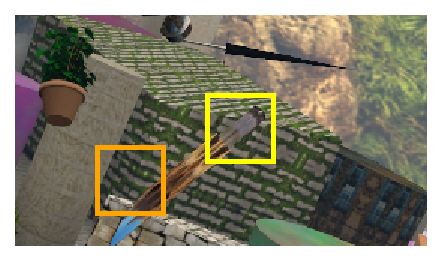
\includegraphics[width=\textwidth]{paper/latex/figures/multiscale_importance_image_patches.pdf}\\
        \vspace{-15pt}                
    \end{subfigure} 
}
\centering
\makebox[\textwidth][c]{
    \begin{subfigure}[b]{1.15\textwidth}
        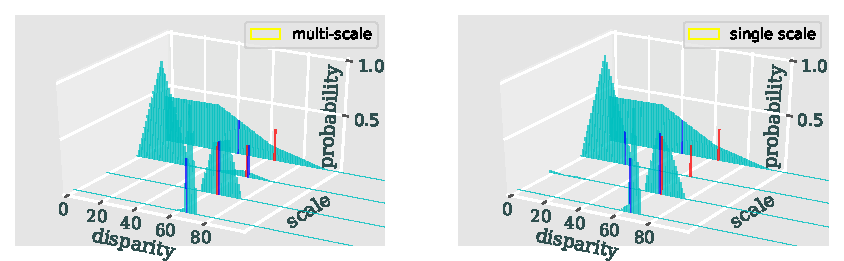
\includegraphics[width=\textwidth]{paper/latex/figures/multiscale_importance_graph_high_resolution.pdf}\\
        \vspace{-15pt}                
    \end{subfigure} 
}
\centering
\makebox[\textwidth][c]{
    \begin{subfigure}[b]{1.15\textwidth}
        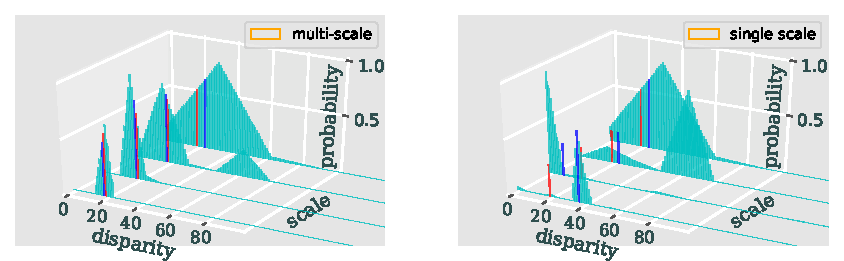
\includegraphics[width=\textwidth]{paper/latex/figures/multiscale_importance_graph_low_resolution.pdf}\\
        \vspace{-15pt}                
        \caption{In this figure, we compare two regions of the same image that require processing on different scale. The centre point of the yellow rectangle is a small object on the foreground with many features (i.e. handle of a knife), whilst the orange one represents a background area inside a repetitive pattern. The first column of graphs represents the Multi-Scale similarity volumes $S^{\{ \sigma_0, ..., \sigma_n \} }$ The graphs prove that, as we expected, disparity estimation is accurate on higher scale for the yellow rectangle and on t As expected,  }
    \end{subfigure} 
}
\vspace{-15pt}
\caption{TEXT}
\label{fig:multiscale_importance}  
\vspace{-3pt}      
\end{figure*}
%%%%%%%%%%%%%%%%%%%%%%%%%%%%%%%%%%%%%%%%%%%%%%%%%%%%%%%%%%%%%%%%
%%%%%%%%%%%%%%%%%%%%%%%%%%%%%%%%%%%%%%%%%%%%%%%%%%%%%%%%%%%%%%%%


%%%%%%%%%%%%%%%%%%%%%%%%%%%%%%%%%%%%%%%%%%%%%%%%%%%%%%%%%%%%%%%%
%%%%%%%%%%%%%%%%%%%%%%%%%%%%%%%%%%%%%%%%%%%%%%%%%%%%%%%%%%%%%%%%
\begin{figure*}[t]
\centering
\makebox[\textwidth][c]{
    \begin{subfigure}[b]{0.28\textwidth}
        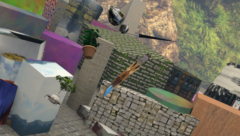
\includegraphics[width=\textwidth]{paper/latex/figures/imL_0.png}\\
        \vspace{-15pt}                
        \caption{$X^{L,1}$}
    \end{subfigure} 
    \hspace{0.001cm} 
    \begin{subfigure}[b]{0.28\textwidth}
        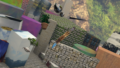
\includegraphics[width=\textwidth]{paper/latex/figures/imL_1.png}\\
        \vspace{-15pt}      
        \caption{$X^{L,2}$}
    \end{subfigure} 
    \hspace{0.001cm} 
    \begin{subfigure}[b]{0.28\textwidth}
        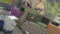
\includegraphics[width=\textwidth]{paper/latex/figures/imL_2.png}\\
        \vspace{-15pt}                      
        \caption{$X^{L,4}$}
    \end{subfigure} 
    \hspace{0.001cm} 
    \begin{subfigure}[b]{0.28\textwidth}
        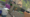
\includegraphics[width=\textwidth]{paper/latex/figures/imL_3.png}\\
        \vspace{-15pt}     
        \caption{$X^{L,8}$}
    \end{subfigure}         
}
\centering
\makebox[\textwidth][c]{
    \begin{subfigure}[b]{0.28\textwidth}
        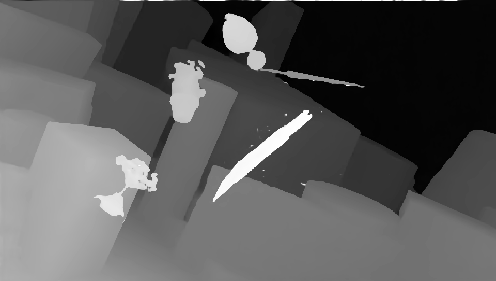
\includegraphics[width=\textwidth]{paper/latex/figures/pred_comb_0.png}\\
        \vspace{-15pt}                
        \caption{$\hat{D}_{comb}^{L,1}$}
    \end{subfigure} 
    \hspace{0.001cm} 
    \begin{subfigure}[b]{0.28\textwidth}
        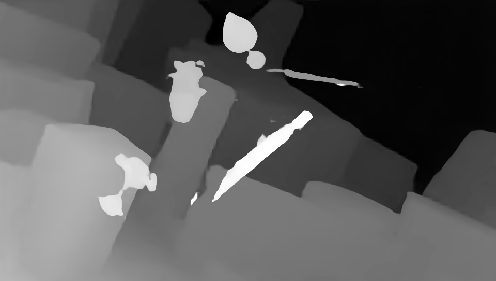
\includegraphics[width=\textwidth]{paper/latex/figures/pred_comb_1.png}\\
        \vspace{-15pt}      
        \caption{$\hat{D}_{comb}^{L,2}$}
    \end{subfigure} 
    \hspace{0.001cm} 
    \begin{subfigure}[b]{0.28\textwidth}
        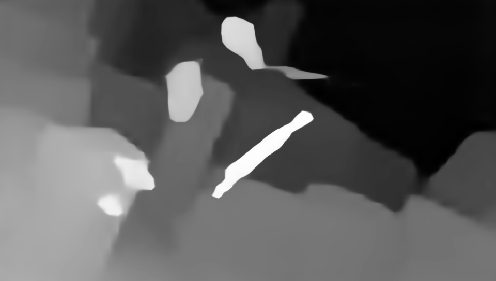
\includegraphics[width=\textwidth]{paper/latex/figures/pred_comb_2.png}\\
        \vspace{-15pt}                      
        \caption{$\hat{D}_{comb}^{L,4}$}
    \end{subfigure} 
    \hspace{0.001cm} 
    \begin{subfigure}[b]{0.28\textwidth}
        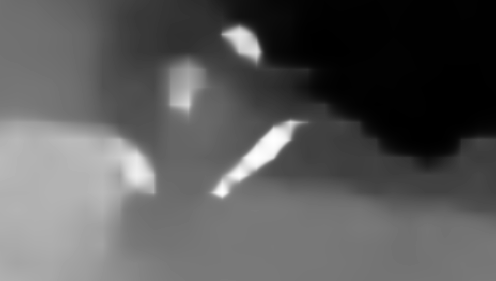
\includegraphics[width=\textwidth]{paper/latex/figures/pred_comb_3.png}\\
        \vspace{-15pt}     
        \caption{$\hat{D}_{comb}^{L,8}$}
    \end{subfigure}         
}
\centering
\makebox[\textwidth][c]{
    \begin{subfigure}[b]{0.28\textwidth}
        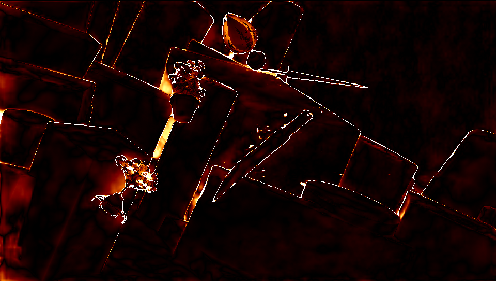
\includegraphics[width=\textwidth]{paper/latex/figures/pred_comb_0_err.png}\\
        \vspace{-15pt}                
        \caption{$E_{comb}^{L,1}$}
    \end{subfigure} 
    \hspace{0.001cm} 
    \begin{subfigure}[b]{0.28\textwidth}
        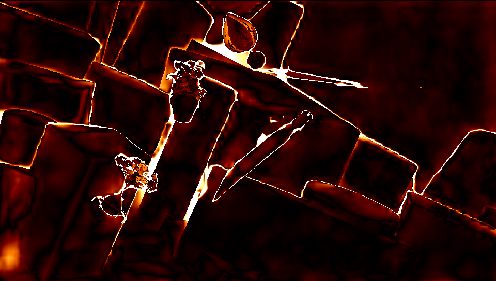
\includegraphics[width=\textwidth]{paper/latex/figures/pred_comb_1_err.png}\\
        \vspace{-15pt}      
        \caption{$E_{comb}^{L,2}$}
    \end{subfigure} 
    \hspace{0.001cm} 
    \begin{subfigure}[b]{0.28\textwidth}
        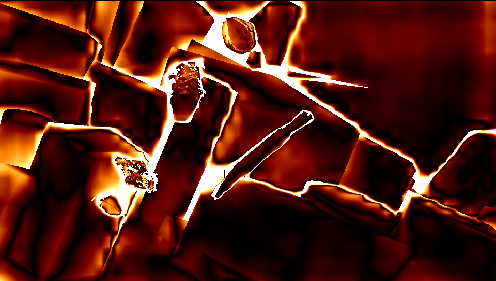
\includegraphics[width=\textwidth]{paper/latex/figures/pred_comb_2_err.png}\\
        \vspace{-15pt}                      
        \caption{$E_{comb}^{L,4}$}
    \end{subfigure} 
    \hspace{0.001cm} 
    \begin{subfigure}[b]{0.28\textwidth}
        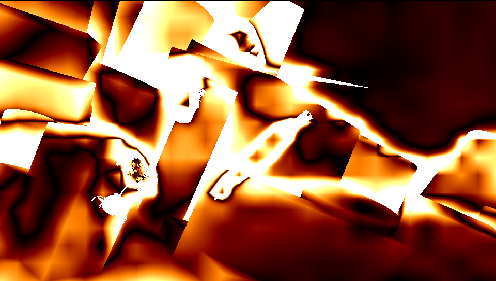
\includegraphics[width=\textwidth]{paper/latex/figures/pred_comb_3_err.png}\\
        \vspace{-15pt}     
        \caption{$E_{comb}^{L,8}$}
    \end{subfigure}         
}
\centering
\makebox[\textwidth][c]{
    \begin{subfigure}[b]{0.28\textwidth}
        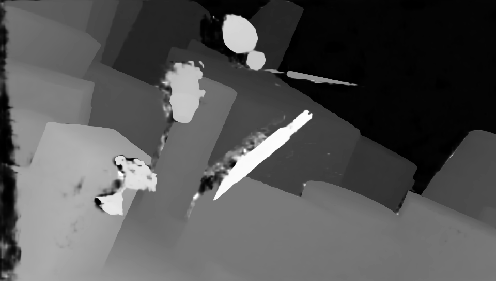
\includegraphics[width=\textwidth]{paper/latex/figures/pred_0.png}\\
        \vspace{-15pt}                
        \caption{$\hat{D}^{L,1}$}
    \end{subfigure} 
    \hspace{0.001cm} 
    \begin{subfigure}[b]{0.28\textwidth}
        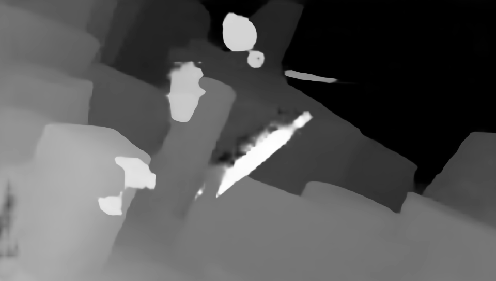
\includegraphics[width=\textwidth]{paper/latex/figures/pred_1.png}\\
        \vspace{-15pt}      
        \caption{$\hat{D}^{L,2}$}
    \end{subfigure} 
    \hspace{0.001cm} 
    \begin{subfigure}[b]{0.28\textwidth}
        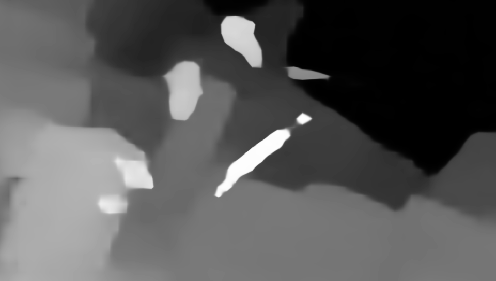
\includegraphics[width=\textwidth]{paper/latex/figures/pred_2.png}\\
        \vspace{-15pt}                      
        \caption{$\hat{D}^{L,4}$}
    \end{subfigure} 
    \hspace{0.001cm} 
    \begin{subfigure}[b]{0.28\textwidth}
        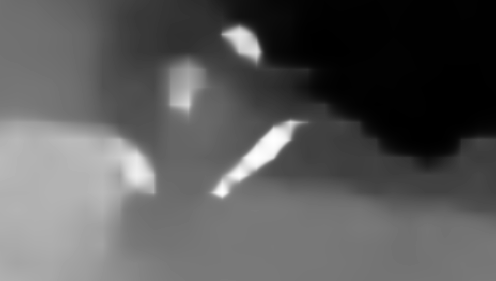
\includegraphics[width=\textwidth]{paper/latex/figures/pred_3.png}\\
        \vspace{-15pt}     
        \caption{$\hat{D}^{L,8}$}
    \end{subfigure}         
}
\centering
\makebox[\textwidth][c]{
    \begin{subfigure}[b]{0.28\textwidth}
        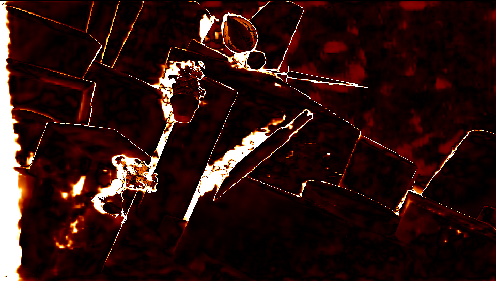
\includegraphics[width=\textwidth]{paper/latex/figures/pred_0_err.png}\\
        \vspace{-15pt}                
        \caption{$E^{L,1}$}
    \end{subfigure} 
    \hspace{0.001cm} 
    \begin{subfigure}[b]{0.28\textwidth}
        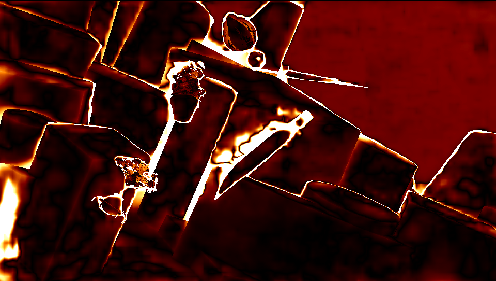
\includegraphics[width=\textwidth]{paper/latex/figures/pred_1_err.png}\\
        \vspace{-15pt}      
        \caption{$E^{L,2}$}
    \end{subfigure} 
    \hspace{0.001cm} 
    \begin{subfigure}[b]{0.28\textwidth}
        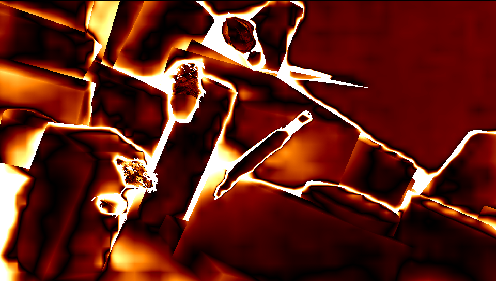
\includegraphics[width=\textwidth]{paper/latex/figures/pred_2_err.png}\\
        \vspace{-15pt}                      
        \caption{$E^{L,4}$}
    \end{subfigure} 
    \hspace{0.001cm} 
    \begin{subfigure}[b]{0.28\textwidth}
        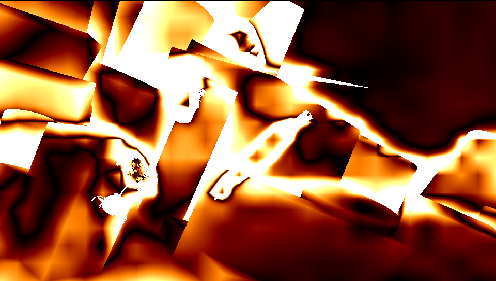
\includegraphics[width=\textwidth]{paper/latex/figures/pred_3_err.png}\\
        \vspace{-15pt}     
        \caption{$E^{L,8}$}
    \end{subfigure}         
}
\vspace{-15pt}
\caption{TEXT}
\label{fig:EMAPs}  
\vspace{-3pt}      
\end{figure*}
%%%%%%%%%%%%%%%%%%%%%%%%%%%%%%%%%%%%%%%%%%%%%%%%%%%%%%%%%%%%%%%%

\subsection{SceneFlow benchmark} \label{sec:4_2}

\subsubsection{Using multi-scale processing implicitly vs explicitly}

In this section, we want to test the benefit of enforcing multi-scale processing explicitly. For this reason, we design 4 CNN architectures that follow the MSNet designing principles, but without enforcing multi-scale processing explicitly; OneRes operates only on the initial resolution, MRes2d uses the hourglass model (i.e. downsampling and upsampling) only in the 2D-processing part, MRes3d uses the hourglass model only in the 3D-processing part and finally MRes2d3d in both the 2D and 3D processing part. The hourglass architecture allows by design implicit multi-scale processing. For each of the 4 CNNs we create two versions; small (S) has the same number of free parameters as MSNet and big (B) which has as many parameters as the GPU memory allows.

In figure \ref{fig:mae_SFNvsSFN_free_weights} we observe that MSNet outperforms both versions of the generic architectures, which is a crucial indicator that enforcing multi-scale processing explicitly is beneficial for depth estimation. More specifically, big (B) networks outperform small (S) ones and using the hourglass architecture in the 3D processing part (MRes3d) gives the best performance.

\begin{figure}[h]
    \centering
    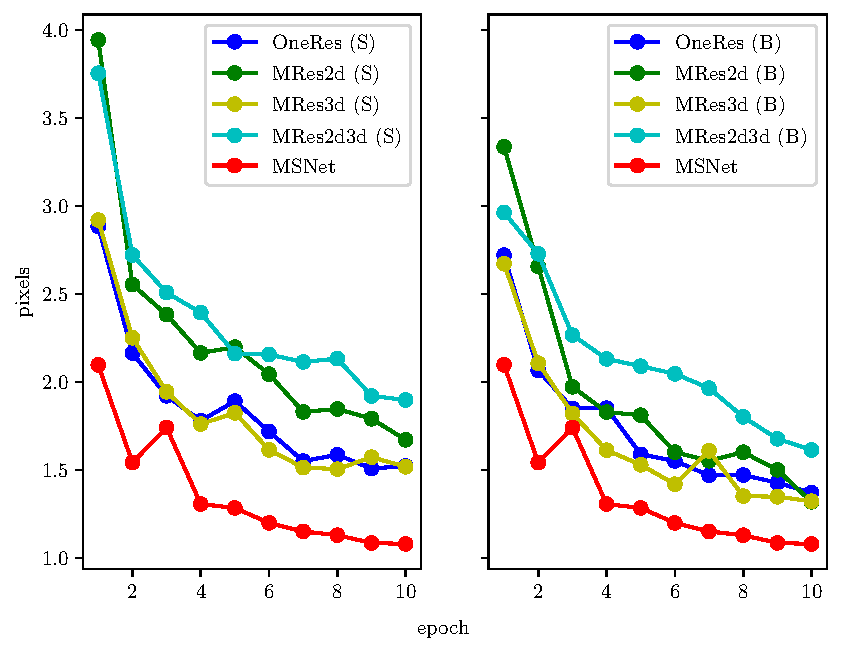
\includegraphics[width=\textwidth]{paper/latex/figures/freiburg_msnet_vs_monolithic_mae.pdf}
    \caption{MSNet comparison with generic architectures}
    \label{fig:mae_SFNvsGenericNets}
\end{figure}

\subsubsection{Comparing MSNet with networks that do not share weights}

In this section, we 

\begin{figure}[t]
    \centering
    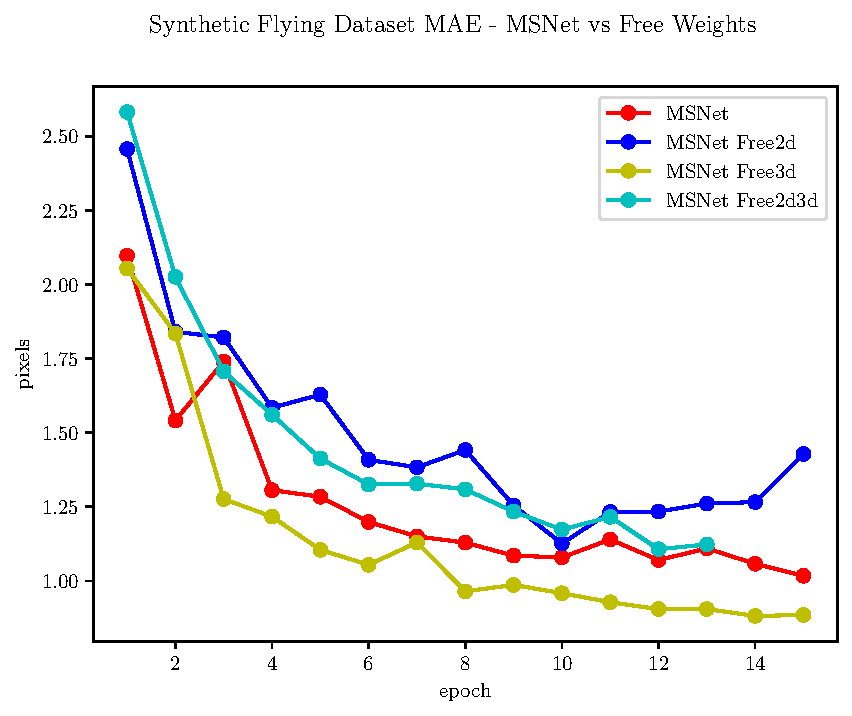
\includegraphics[width=\textwidth]{paper/latex/figures/freiburg_msnet_vs_free_weights_mae.pdf}
    \caption{Text}
    \label{fig:mae_SFNvsSFN_free_weights}
\end{figure}

Secondly, we question whether using the same constructive blocks $f_1$, $f_2$, $f_3$, $f_4$ repetitively between different scales lead to better results that leaving all model weights free along training. We must notice here that freeing the weights cancels the networks scalability, since the processing scales must be predefined and be consistent between training and test phase. From the results at table \ref{tab:results} and figure \ref{fig:mae_SFNvsSFN_free_weights} we can extract two conclusions; Firstly, training the network $f_1$ once for all scales leads to an optimal solution. Seconly, at the 3d level, repeating the building block $f_2$ and $f_3$ through MultiScaleFusion algorithm \ref{alg:multi_scale_fusion} leads to suboptimal solution. Keeping the same backbone architecture, with free weights between scales, provides better accuracy in the cost of $4x$ parameters and the cancelling of scalability.

\subsubsection{Compare MSNet vs state-of-the-art networks}

Finally, we compare our network with the SoA models. In table \ref{tab:results}, it is shown that MSNet and MSNetFree3d set a new state-of-the-art performance. MSNet, specifically, the SoA performance even though it is much lighter network than those presented in previous works.

\begin{table}[]
    \centering
    \begin{tabular}{ c|c|c|c|c }
    Method & Parameters (M) & Runtime & MAE & PCG \\
    
    \hline
    \multicolumn{5}{c}{ \textbf{Our benchmark - Generic nets} } \\
    \hline
    MSNet & 0.743 & 0.32 & 1.017 & 3.98 \\
    \hline
    OneRes (S) & 0.463 & 0.11 & 1.508 & 6.11 \\
    MRes2d (S) & 0.659 & 0.10 & 1.671 & 6.98 \\
    MRes3d (S) & 0.514 & 0.15 & 1.504 & 5.86 \\
    MRes2d3d (S) & 0.677 & 0.3 & 1.897 & 8.078 \\
    \hline
    OneRes (B) & 1.608 & 0.22 & 1.37 & 5.53 \\
    MRes2d (B) & 1.458 & 0.17 & 1.32 & 5.43 \\
    MRes3d (B) & 1.682 & 0.21 & 1.322 & 5.11 \\
    MRes2d3d (B) & 1.772 & 0.32 & 1.613 & 6.67 \\
    \hline
    \multicolumn{5}{c}{ \textbf{Our benchmark - Free weights} } \\
    \hline
    Free2d & 0.969 & 0.24 & 1.126 & 4.33 \\
    Free3d & 2.75 & 0.33 & \textbf{0.882} & \textbf{3.48} \\
    Free2d3d & 2.974 & 0.33 & 1.107 & 4.36 \\
    \hline
    \multicolumn{5}{c}{ \textbf{SoA} } \\
    \hline
    PSMNet\cite{Chang2018PyramidNetwork} & - & - & 1.09 & - \\
    CRL\cite{Pang2018CascadeMatching} & - & - & 1.32 & - \\
    DispNetC\cite{Mayer2016ALD} & - & - & 1.68 & - \\
    GC-Net\cite{Kendall2017End-to-EndRegression} & 3.5 & 0.95 & 2.51 & 9.34 \\
    
    \hline
    \end{tabular}
    \caption{Model comparison on SceneFlow dataset}
    \label{tab:results}
\end{table}

\subsubsection{MSNet evaluation on smaller training set}

In figure \ref{fig:msnet_smaller_tr_set}, it is shown how MSNet observes when trained on a smaller percentage of the training set. As expected, the accuracy increases as the model observes more training data.

\begin{figure}
    \centering
    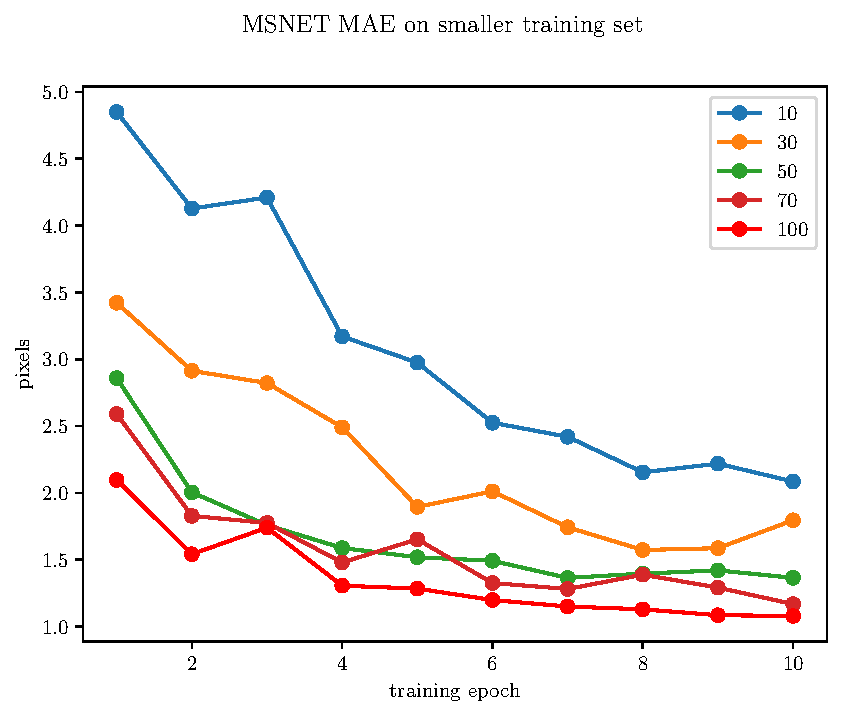
\includegraphics[width=\textwidth]{paper/latex/figures/freiburg_msnet_mae_smaller_training_set.pdf}
    \caption{Caption}
    \label{fig:msnet_smaller_tr_set}
\end{figure}{}

\subsubsection{MSNet evaluation on different scale combinations}

In figure \ref{fig:msnet_scales_evaluation}, we evaluate MSNet under different scale combinations. We observe that not only error in terms of $\mu$ absolute error and PCG error decreases as we add more scales, but also the standard deviation $\sigma$. This indicates that our network becomes more robust by operating in more scales. We also observe that adding coarse scales increases the robustness, even though the accuracy may be worse; for example $T=\{ 8 \}$ is better than $ T = \{ 16 \}$ in terms of accuracy (i.e. smaller $\mu$ absolute error) but $ T = \{ 16 \}$ is more robust (i.e. smaller $\sigma$). 

\begin{figure}
    \centering
    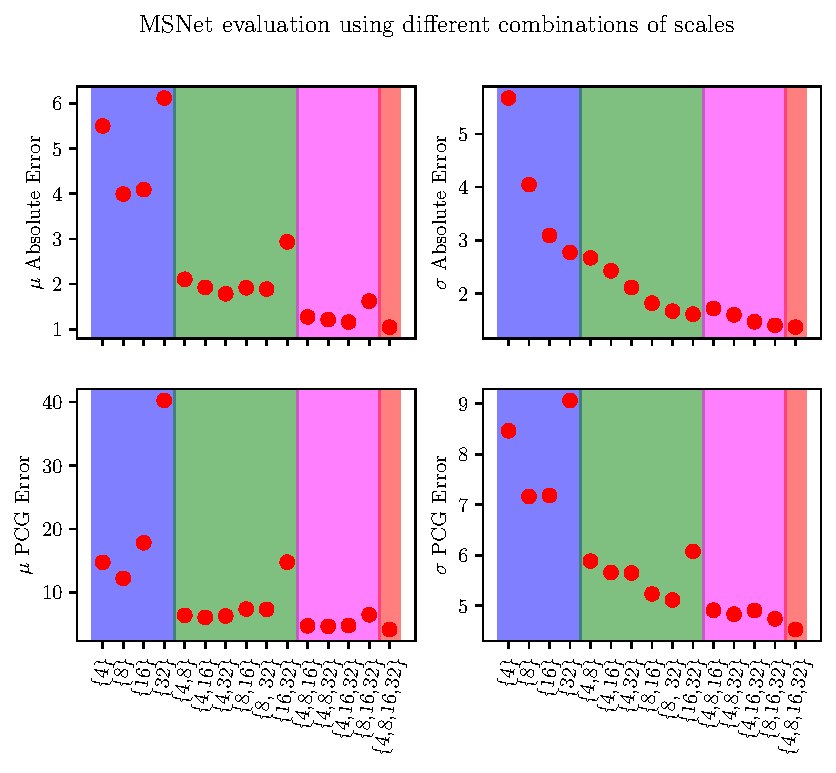
\includegraphics[width=\textwidth]{paper/latex/figures/msnet_scales_evaluation.pdf}
    \caption{MSNet accuracy for different scale combinations. On the x-axis, there are the different scale combinations (i.e. the blue area contains single-scale set-ups, the green area two-scale, the purple area three-scale and the orange area the four-scale combination that was used in the training phase). On the first row we observe the $\mu$ and $\sigma$ of the absolute end-point error and on the second row the $\mu$ and $\sigma$ of the percentage of points with end-point error over 3 pixel.}
    \label{fig:msnet_scales_evaluation}
\end{figure}


%%%%%%%%%%%%%%%%%%%%%%%%%%%%%%%%%%%%%%%%%%%%%%%%%%%%%%%%%%%%%%%%
%%%%%%%%%%%%%%%%%%%%%%%%%%%%%%%%%%%%%%%%%%%%%%%%%%%%%%%%%%%%%%%%





%%%%%%%%%%%%%%%%%%%%%%%%%%%%%%%%%%%%%%%%%%%%%%%%%%%%%%%%%%%%%%%%

\section{Conclusions}


\bibliographystyle{plain}
\bibliography{bibliography.bib}

\end{document}
